%!TEX root = ../main.tex

\chapter{Results\label{chap:results}}
\alertwarning{under construction}

\mycomment{% %%{
    This section describes experiments and evaluation of performance of the proposed method for mapping of ionizing radiation.
    An experiment with real sources of ionizing radiation requires (due to specific safety measures, permission from the state authorities...) coordination with other institutions, such as Czech metrology institute.
    Unfortunately, it was not possible to perform experiment with real sources before the deadline of the thesis due to these organizational reasons.
    However, the method was evaluated on pre-recorded data from real-world experiments as well as using the realistic simulator for compton camera \cite{TODO}.
}% %%}

\section{Monte carlo simulation results}
In figure \ref{fig:monte_cs_results}, the probability of a Cesium-137 photon generating a Compton cone when emitted from a distance of 1 meter is displayed. 
The sensor's sensitivity is observed to be nearly uniform regardless of the incoming particle's direction. 
This outcome can be explained using Figure \ref{fig:monte_clar}. 
As illustrated in figure \ref{fig:monte_reaching}, particles that approach the sensor from the front side have a greater visible surface area, resulting in a greater likelihood of hitting the sensor. 
Conversely, particles arriving from the side have a longer intersection with the sensor's material, resulting in a greater probability of producing a Compton cone, as shown in figure \ref{fig:monte_cone_from_hitting}. 
Surprisingly, these two effects compensate for each other, resulting in an almost consistent sensitivity of the sensor to particles arriving from various directions.

\begin{figure}[!htb]
  \centering
  \subfloat {
    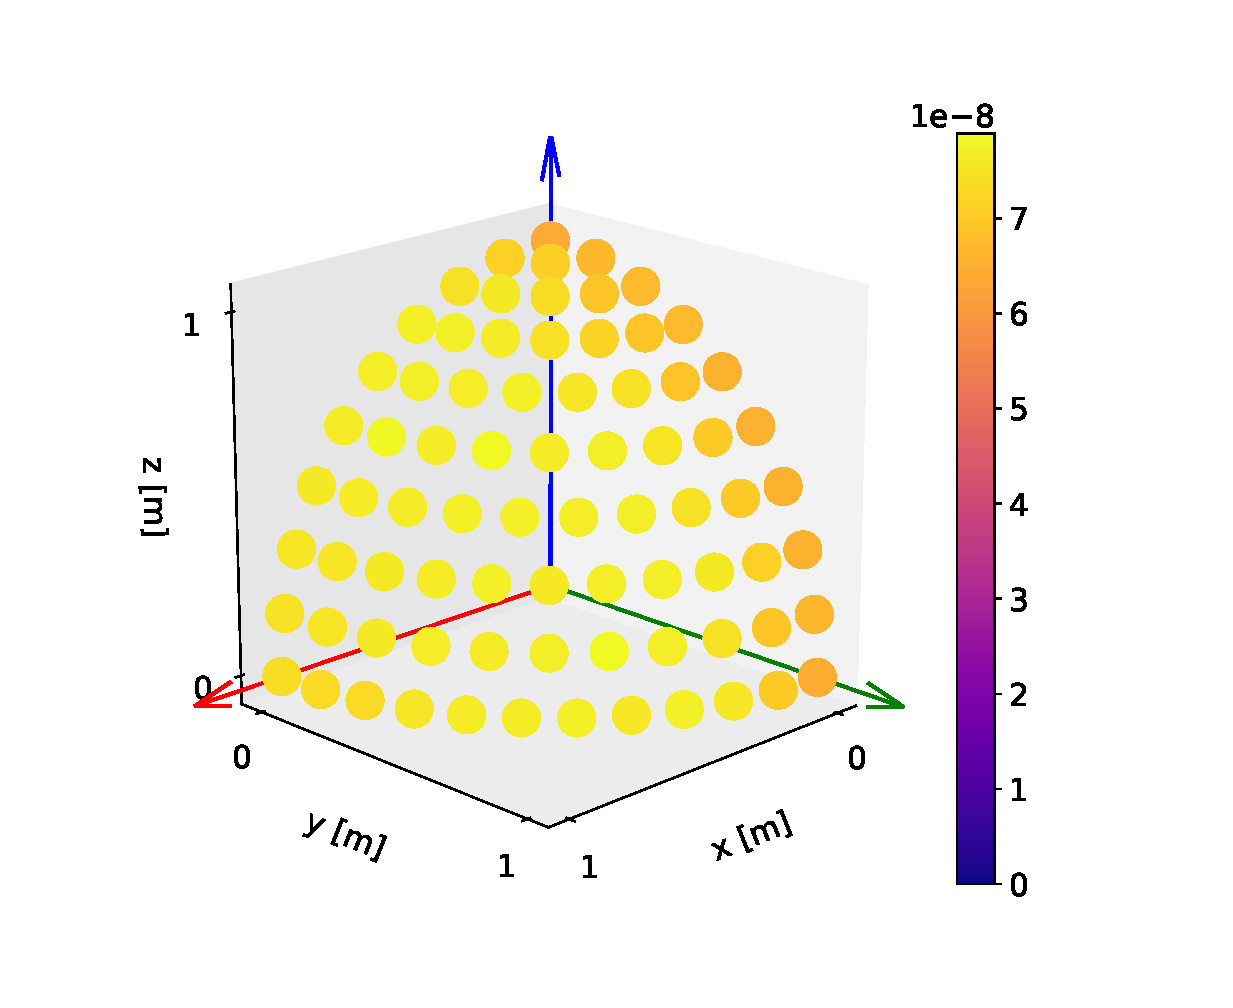
\includegraphics[width=0.7\textwidth]{./fig/photos/mc_cs_prob_compton.eps}
  }
  \caption{Probability that particle emitted at certain position produces a compton cone.}
  \label{fig:monte_cs_results}
\end{figure}

\begin{figure}[!htb]
  \centering
  \subfloat[Probability of reaching the surface] {
    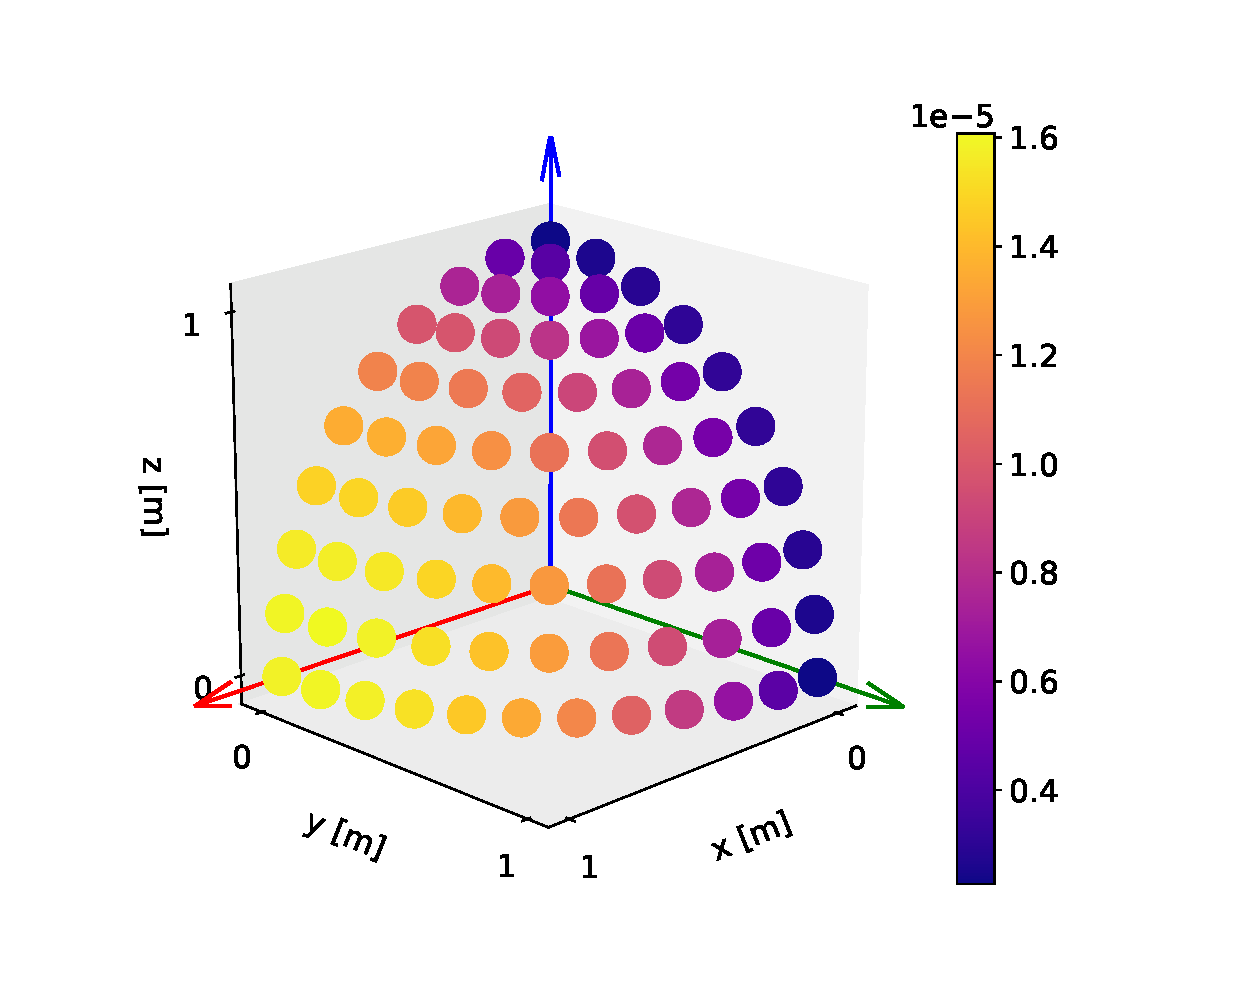
\includegraphics[width=0.5\textwidth]{./fig/photos/mc_prob_reaching_the_surface.eps}
    \label{fig:monte_reaching}
  }
  \subfloat[probability that particle hitting the sensor produce a compton cone.] {
    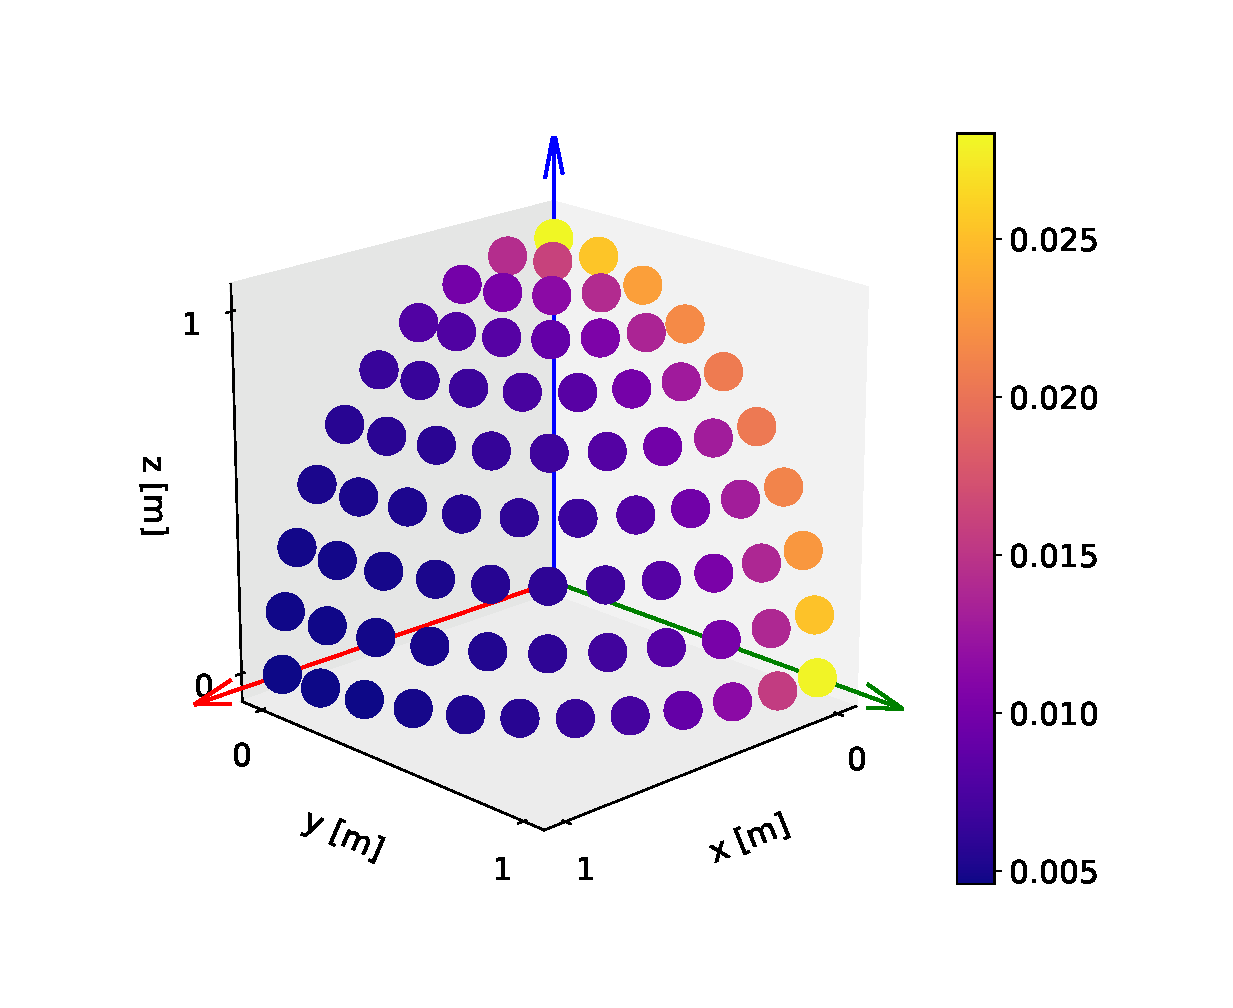
\includegraphics[width=0.5\textwidth]{./fig/photos/mc_comptons_from_sensor_hits.eps}
    \label{fig:monte_cone_from_hitting}
  }
  \caption{Results of Monte carlo simulation for cs137.}
  \label{fig:monte_clar}
\end{figure}

\section{Evaluation on recorded real-world data}
TODO
\section{Simulations in gazebo}

\section{Real-world experiment with simulated sources}

\subsection{Experimental setup}
The radiation mapping pipeline was tested on a real hardware during the field experiments.
Three \ac{UAV} were used during this experiment.
The real radioactive sources were replaced with simulated ones, the Compton camera simulator \cite{TODO} was running onboard each \ac{UAV}.
All the drones were localized using \ac{gps} in the same coordinate frame and the positions of simulated sources were shared among them.
The size of mapped area was set to $100 \times 100$ m, four simulated sources with activities 500 MBq, 1 GBq, 2 GBq and 2 GBq were placed in the area.
Resolution of the map was $0.5$ m.

\subsection{Results}
\begin{table}[htb]
\begin{center}
  \begin{tabular}{ |c|c|c|c| } 
 \hline
    \multicolumn{2}{|c}{Sources} &  \multicolumn{2}{|c|}{ relative activity } \\
 \hline
    position & activity & ground truth & MLEM estimate\\ 
 \hline
    (10, 20) & 2000 MBq & 1.0  & \textbf{1.0} \\ 
    (20, 20) & 1000 MBq &  0.5 & \textbf{0.49} \\ 
    (80, 80) & 1000 MBq &  0.5 & \textbf{0.52} \\ 
    (75, 75) & 500 MBq &  0.25 & \textbf{0.0} \\ 
 \hline
\end{tabular}
  \caption{Results of the real world experiment with simulated data. Last column presents estimated relative activity at the map positions that correspond to the ground truth position of the given source.}
  \label{tab:temenight_results}
\end{center}
\end{table}











\mycomment{% %%{




    \section{Pre-recorded data with real radioactive sources}


    \section{Gazebo simulations with the simulated Compton camera}

    \section{Real-world experiment with the simulated Compton camera}



    The approach presented in the previous section was applied on a prerecorded rosbag from a real-world experiment.
    Four \ac{UAV}s were used in this experiment.
    The mapped area was $50 \times 35$ meters with $0.4$ m resolution.
    The experiment took approximately 8 minutes and 250 cones were measured.

    The estimated vector of $\bf{\lambda}$ is presented in figure \ref{fig:D}. 
    The ground truth positions of radioactive sources with their strength can be seen on figure \ref{fig:C}.
    The sensitivity vector $\mathbf{s}$ and the matrix $\mathbf{T}$ summed over all measurements (which serves as simple projection of the cones to the map) are presented in figures \ref{fig:E} and \ref{fig:F}.
    \begin{figure}[!h]
      \centering
      \subfloat[True positions of sources (MBq)] {
        
\includegraphics[width=0.5\textwidth]{./fig/photos/temenight_ground_truth.eps}
        \label{fig:C}
      }
      \subfloat[MLEM estimate after 10 iterations] {
        
\includegraphics[width=0.5\textwidth]{./fig/photos/temenight_lambdas.eps}
        \label{fig:D}
      }
      \label{fig:A}
      \caption{Comparison of \ac{MLEM} algorithm estimate and the ground truth.}
    \end{figure}

    \begin{figure}[!htb]
      \centering
      \subfloat[System matrix $\mathbf{T}$ summed over $\forall i$] {
        
\includegraphics[width=0.5\textwidth]{./fig/photos/temenight_back_projection.eps}
        \label{fig:E}
      }
      \subfloat[Sensitivity vector $\mathbf{s}$] {
        
\includegraphics[width=0.5\textwidth]{./fig/photos/temenight_sensitivity.eps}
        \label{fig:F}
      }
      \label{fig:B}
      \caption{System matrix and sensitivity vector estimated during the experiment}
    \end{figure}

    \section{Discussion}
    We can see that the algorithm precisely detected the 500 MBq source. Two smallest source were not recognised, probably due to low number of cones measured.
    The 1900 MBg source was partially detected. 
    In is important to note that the drones were flying mostly around the 500 MBg source and most of the measured cones originated from that source, as we can see in the sensitivity vector and system matrix.
    This approach seems to be beneficial compared to naive back-projection of the cones to the map (without weighting with the sensitivity), since it can "see" the 1900 MBq source despite the fact that only few cones originated there.


}% %%}
